\documentclass[notes]{beamer}
\usetheme{Boadilla}
\usepackage{eqnarray, amsmath}
\usepackage{amssymb}
\usepackage{soul}
\usepackage{caption}
\usepackage{xcolor,colortbl}
\setbeamertemplate{caption}[numbered]
\usepackage{subcaption}
\usepackage{bbm}
\usepackage{graphicx}
\usepackage{pgfpages}
\setbeamertemplate{note page}[plain]
\usepackage{pgfpages}
\usepackage{amsmath}
\usepackage[round]{natbib}  
%\setbeameroption{show only notes}
\DeclareMathOperator*{\argmin}{arg\,min}
\usepackage[utf8]{inputenc}
\title{Teacher Turnover and Student Performance: Evidence from Pennsylvania Public Schools}
\author{Collin Wardius}
\institute{Temple University}
\date{April 16th, 2020}

\begin{document}
\begin{frame}
\titlepage
\end{frame}

\begin{frame}{Introduction}
\doublespacing
\begin{enumerate}[I]
    \item More \textit{new} teachers are leaving the profession. \cite{watlington}
    \begin{enumerate}[i]
        \item 50\% of teachers leave in their first five years.
    \end{enumerate}
 \item More teachers \textit{of any} experience level are leaving the profession. \cite{hammond}
 \begin{enumerate}[i]
    \item 5.1\% of teachers left the profession in 1994. 8.4\% left in 2005.
    \item $\approx 90,000$ additional positions to fill 
\end{enumerate}
\end{enumerate}
\end{frame}

\note{
\begin{enumerate}
    \item The text is pretty self-explanatory
    \item I would only note that teacher's leaving more frequently is only an issue if it negatively effects performance. Otherwise, we should be ok with this phenomenon
\end{enumerate}
}

\begin{frame}{Introduction}
\doublespacing
\textbf{Question: Is teacher turnover causally related to student performance?}
\end{frame}



\begin{frame}{Literature Review}
\begin{enumerate}[I]
    \item Two types of turnover effects:
    \begin{enumerate}[i]
        \item Compositional effects--effects on the composition of experience and talent of teaching faculty.
        \item Disruptive effects--effects on schools generally.
        \begin{enumerate}
            \item Hiring costs
            \item Faculty cohesion
            \item Inexperience
        \end{enumerate}
    \end{enumerate}
    \item \cite{ronfeldt}
    \begin{enumerate}[i]
        \item 4th and 5th grade. NYC Public Schools
        \item Teacher Turnover $\uparrow$ $\rightarrow$ Performance (Math/English) $\downarrow$.
    \end{enumerate}
    \item \cite{adnot}
    \begin{enumerate}[i]
        \item Washington D.C. Public Schools
        \item IMPACT just implemented (dismiss ineffective teachers)
        \item No statistically significant effect of teacher turnover
    \end{enumerate}
\end{enumerate}  
\end{frame}
\note{
\begin{enumerate}
    \item Example of compositionl effect: if old and uncaring teachers are replaced by young and passionate teachers, this is a positive compositional effect. Alternatively, if experienced teachers are replaced by inexprienced teachers, this is a negative compositional effect.
    \item IMPACT is a program that evaluates teachers on different metrics and seeks to dismiss ineffective teachers. Therefore, turnover in the Adnot study is actually being caused by some mechanism external to the teachers themselves.
\end{enumerate}
}


\begin{frame}{Data}
\begin{enumerate}[I]
    \item Years: 2014 to 2018
    \item Source: Pennsylvania Department of Education
    \begin{enumerate}[i]
        \item Pennsylvania System of School Assesment (PSSA) performance measures
        \item Enrollment data
        \item Teacer-level data
        \item Expenditure data
    \end{enumerate}
\end{enumerate}
\end{frame}
\note{
\begin{enumerate}
    \item The PSSA is a standardized test taken in grads 3-8 in math and English and in grades 4 and 8 in science. The PSSA gauges whether students are making adequate learning progress and helps schools identify students who need additional assistance. It also helps schools gauge whether special needs students are meeting learning goals as specified in their Individualized Education Plan. 
    \item Teacher-level data includes school assignment, years of experience, education level, and salary.
\end{enumerate}
}


\begin{frame}{Data}
\centering
\begin{figure}[ht]
            \centering
            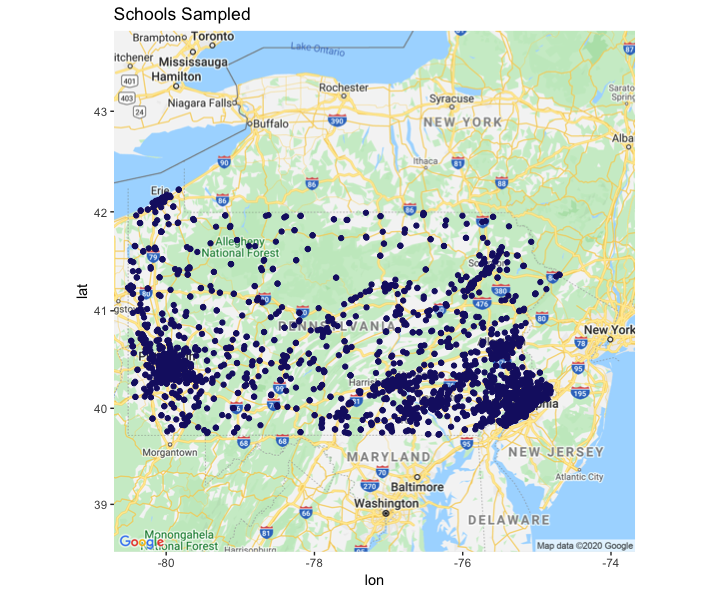
\includegraphics[scale=.3]{school_sample.png}
            \caption{Schools in Sample (2014-2018)}
            \label{fig:my_label}
\end{figure}
\end{frame}

\begin{frame}{Data}
\centering
\begin{figure}[ht]
\centering
         
         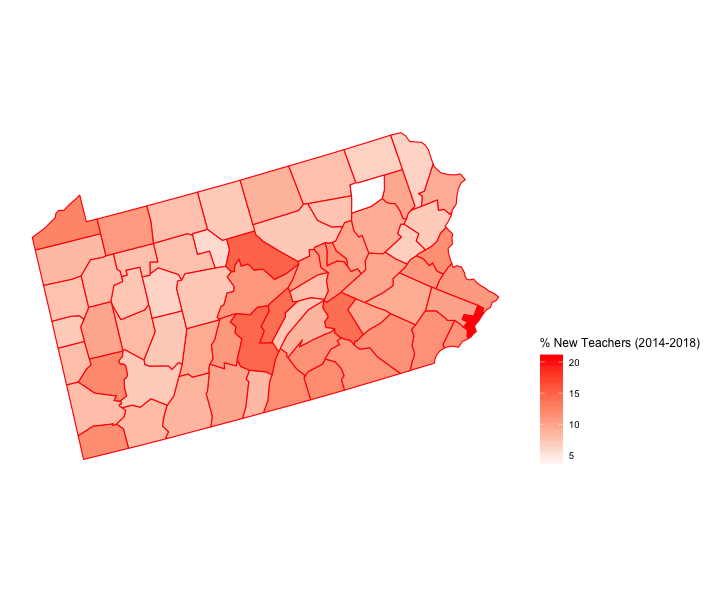
\includegraphics[scale=.3]{turnover_heatplot.png}
            \caption{Turnover by County}
            \label{fig:my_label}
\end{figure}
\end{frame}
\note{
\begin{enumerate}
    \item Turnover is most prevalent in urban counties. See Philadelphia and Allegheny counties.
\end{enumerate}

}



\begin{frame}{Data}
\begin{table}[htbp]\centering
\tiny
\def\sym#1{\ifmmode^{#1}\else\(^{#1}\)\fi}
\caption{Summary Statistics, Pennsylvania Department of Education and American Community Survey Data from 2014 to 2018.}
\begin{tabular}{l*{1}{cccc}}
\hline\hline

                    &  Mean&          SD&         Min&         Max\\
\hline
\textit{Control Variables} \\
\hline
\rule{0pt}{4ex}Percent of New Teachers&   11.33&       11.28&        0.00&      100.00\\
Teacher to Student Percent&    7.49&        1.72&        0.19&       34.04\\
Admin. to Student Percent& .32&        0.19&        0.00&        2.60\\
Exp. Per Student (\$1000)&   18.21&     4.43&     8.38&    60.50\\
County Med. Income (\$1000)&    28.34&     5.04&    14.88&    41.52\\
\hline
\textit{Performance Measures} \\
\hline
\rule{0pt}{4ex}Math Grade 3        &     53.73&       22.61&        0.00&      100.00\\
Math Grade 4        &    45.10&       22.57&        0.00&      100.00\\
Math Grade 5        &     42.53&       22.62&        0.00&       98.30\\
Math Grade 6        &    36.63&       21.43&        0.00&      100.00\\
Math Grade 7        &      31.72&       19.55&        0.00&       98.00\\
Math Grade 8        &     26.82&       17.85&        0.00&       93.80\\
Science Grade 4     &      75.98&       19.93&        6.30&      100.0\\
Science Grade 8     &   50.73&       22.54&        0.00&      100.00\\
English Grade 3     &    62.87&       20.48&        0.00&      100.00\\
English Grade 4     &       59.80&       21.21&        0.00&      100.00\\
English Grade 5     &      58.68&       21.88&        0.00&      100.00\\
English Grade 6     &     58.87&       21.57&        0.00&      100.00\\
English Grade 7     & 55.18&       20.98&        0.00&      100.00\\
English Grade 8     &     54.10&       21.03&        0.00&      100.00\\
\hline\hline
\end{tabular}
\caption*{\textit{Note:} Data at school-by-academic year level. 2193 schools. 10964 observations.}
\end{table}
\end{frame}
\note{
\begin{enumerate}
    \item Perhaps just point out that there are some unreasonably high observations for percent of new teachers. These are very few and dropping them does not effect the results of the paper, so I keep them in an effort to keep the data as is.
\end{enumerate}

}


\begin{frame}{Model}
$$y_{st} = d_{st}\gamma + x_{st}'\beta + \lambda_s + \delta_t + \epsilon_{st}$$
\begin{enumerate}[I]
\item School-level fixed effects panel data model
    \begin{enumerate}[i]
        \item $y_{st}$: student achievement
        \item $d_{st}$: teacher turnover (the ``treatment")
        \item $x_{st}$: controls (median income, teachers per student,...)
        \item $\lambda_s$: school fixed effects
        \item $\delta_t$: academic year fixed effects
    \end{enumerate}
\end{enumerate}
\end{frame}
\note{
\begin{enumerate}
    \item $s$ indexes school and $t$ indexes time (academic year)
    \item The model exploits within school variation in teacher turnover and pssa performance to estimate $\gamma$
\end{enumerate}

}



\begin{frame}{Results}
\begin{enumerate}[I]
    \item A one percent increase in teacher turnover decreases the expected proportion of students earning advanced or proficient by .05 percentage points.
    \item The result is statistically significant at the .01\% significance level.
    \item Effect of teacher turnover is more pronounced in low income counties.

    \item In the fixed effects model, we do not estimate a statistically significant quadratic effect of teacher turnover.
\end{enumerate}
\end{frame}

\begin{frame}{Results}
\begin{table}[hbtp]
    \tiny
    \centering
    \caption{Relationship Between Proportion of New Teachers and Student Performance}
\begin{tabular}{lcc}
\multicolumn{3}{c}{} \\ \hline\hline
 & (1) & (2) \\
 &  & School FE \\
VARIABLES & Pooled OLS & Cluster SE \\ \hline
 &  &  \\
\rowcolor{yellow}New Teachers to All Teachers Ratio (\%) & -0.51*** & -0.05*** \\
 & (0.02) & (0.01) \\
Teacher to Student Ratio (\%) & 1.72*** & 0.48*** \\
 & (0.14) & (0.09) \\
Administrator to Student Ratio (\%) & -14.02*** & 0.53 \\
 & (1.21) & (0.51) \\
Expenditures Per Student (in \$1000) & -1.00*** & -0.06*** \\
 & (0.05) & (0.02) \\
County Median Income (in \$1000) & 1.57*** & 0.11 \\
 & (0.04) & (0.20) \\
Constant & 20.41*** & 48.27*** \\
 & (1.52) & (5.41) \\
 &  &  \\
\hline
Observations & 8,524 & 8,524 \\
R-squared & 0.30 & 0.06 \\
 Number of Schools & 2,193 & 2,193 \\ \hline\hline
\multicolumn{3}{c}{ Robust standard errors in parentheses} \\
\multicolumn{3}{c}{ *** p$<$0.01, ** p$<$0.05, * p$<$0.1} \\
\end{tabular}
\end{table}
\end{frame}

\note{
\begin{enumerate}
    \item new teachers to all teachers statistic is of primary interest
    \item \textit{school fe cluster se} is the model of primary interest. Inclusion of standard OLS models is customary.
    \item Expenditures per student decreases outcomes. This likely points to omitted variable bias where we are not controlling for factors that vary over time and effect performance.
    \item All other coefficients are as one would expect.
    \item While the effect of turnover is statistically significant, it may not be economically significant. This could be the cause of attenuation bias that is endemic to fixed effects models. Further exploration of this is needed.
    \item $R^2$ is rather low in the fixed effects model. This could be the case because of little variation in either performance or in turnover. We could also control for more factors that influence student performance if the data was more robust. 
\end{enumerate}


}

\begin{frame}{Results: High vs. Low Income Counties}

\begin{table}[hbtp]
    \centering
    \tiny
     \caption{Relationship Between Proportion of New Teachers and Student Performance}
\begin{tabular}{lcc}
\multicolumn{3}{c}{} \\ \hline\hline 
 & (1) & (2) \\
VARIABLES & Low Income & High Income \\ \hline
 &  &  \\
\rowcolor{yellow}New Teachers to All Teachers Ratio (\%) & -0.11** & -0.02* \\
 & (0.05) & (0.01) \\
Teacher to Student Ratio (\%) & 0.33 & 0.14 \\
 & (0.58) & (0.24) \\
Administrator to Student Ratio (\%) & -4.56 & -0.02 \\
 & (2.81) & (1.27) \\
Expenditures Per Student (in \$1000) & -0.42 & 0.01 \\
 & (0.37) & (0.06) \\
County Median Income (in \$1000) & -0.25 & -0.64 \\
 & (1.05) & (0.40) \\
Constant & 66.00** & 87.33*** \\
 & (24.93) & (14.11) \\
 &  &  \\
 \hline
Observations & 208 & 1,576 \\
R-squared & 0.15 & 0.04 \\
 Number of Schools & 52 & 417 \\ \hline\hline
\multicolumn{3}{c}{ Robust standard errors in parentheses} \\
\multicolumn{3}{c}{ *** p$<$0.01, ** p$<$0.05, * p$<$0.1} \\
\end{tabular}
\end{table}
\end{frame}

\note{
\begin{enumerate}
    \item Many of the comments are the same from the firs reults table.
    \item Many statistics fail to be statistically significant now, likely because the sample is too small and there is measurement error in some of the variables. 
    \item The model is substantially better at predicting for low income as compared to high income counties as evidenced by the $R^2$. 
\end{enumerate}
}




\begin{frame}{Results: Quadratic Model}
\begin{table}[hbtp]
    \centering
    \tiny 
    \caption{\textbf{Quadratic} Relationship Between Proportion of New Teachers and Student Performance}
    \begin{tabular}{lcc}
\multicolumn{3}{c}{} \\ \hline\hline 
 & (1) & (2) \\
 &  & School FE \\
VARIABLES & Pooled OLS & Cluster SE \\ \hline
 &  &  \\
\rowcolor{yellow}New Teachers to All Teachers Ratio (\%) & -0.69*** & -0.06*** \\
 & (0.05) & (0.01) \\
\rowcolor{yellow}New Teachers to All Teachers Ratio$\wedge$2 & 0.00*** & 0.00 \\
 & (0.00) & (0.00) \\
Teacher to Student Ratio (\%) & 1.74*** & 0.49*** \\
 & (0.14) & (0.09) \\
Administrator to Student Ratio (\%) & -14.16*** & 0.52 \\
 & (1.20) & (0.51) \\
Expenditures Per Student (in \$1000) & -0.00*** & -0.00*** \\
 & (0.00) & (0.00) \\
County Median Income (in \$1000) & 0.00*** & 0.00 \\
 & (0.00) & (0.00) \\
Constant & 19.93*** & 48.24*** \\
 & (1.53) & (5.41) \\
 &  &  \\
 \hline
Observations & 8,524 & 8,524 \\
R-squared & 0.30 & 0.06 \\
 Number of sid & 2,193  & 2,193 \\ \hline\hline
\multicolumn{3}{c}{ Robust standard errors in parentheses} \\
\multicolumn{3}{c}{ *** p$<$0.01, ** p$<$0.05, * p$<$0.1} \\
\end{tabular}
\end{table}
\end{frame}
\note{
\begin{enumerate}
    \item One can see that the quadratic term is not statistically significant in the FE model. 
\end{enumerate}
}

\begin{frame}{Conclusion}
\begin{enumerate}[I]
    \item There is further evidence that nontargeted teacher turnover has negative effects.
    \item Teacher turnover is an especially pertinent concern in low income areas.
    \item More granular (grade-level) data is needed for a more convincing and precise analysis.
    \item Additional teacher-level attributes would also be helpful (teaching assignment, unique identifier).
\end{enumerate}
    
\end{frame}





\begingroup
\tiny
\begin{frame}{References}
\nocite{*}
\bibliographystyle{plainnat}
\bibliography{mybib.bib}
\end{frame}
\endgroup




\end{document}
